\section{Appendix Simulation Model Description}\label{app:modeldescription}
In this appendix the Cashier management and Vehicle management models will be described in detai. For every couple of modules there are figures and a description of what the modules on that figure do.

\subsection{Cashier Management}\label{app:cashierdescription}
In figure \ref{fig:model-cashier} we find the main model. The first part of the main model can be found in figure \ref{fig:createcheckouts}. 
The first module is $Create \ Checkout$. This module creates at the start of every simulation five checkouts. 
These checkouts are assigned a number from 1 to 5 in the next module, $Assign \ checkout \ numbers$, so we differentiate the checkouts. 
After this these five checkouts will remain in $Seize \ Cashier$ until a cashier is available in the model. 
The model has 12 different resources, each which represents a shift. In every shift it is stated when and for how long cashiers will work. 
These cashiers are put as resources in the set $Cashiers$, when there are available cashiers in this set a checkout will seize one and continue in the model. 
The last two modules are the $OnChange$ and $Assign \ Duplicate \ Checkoutnumber$ which do the same as the first two modules, only now for duplicate checkout entities. 
The $OnChange$ is triggered when a cashier is almost finished working his shift as mentioned above. 
This is necessary because when a single cashier is done working his shift, the checkout entity will leave the model and we need another entity which is exactly the same as the one leaving the system. 
Therefor the duplicate entity.

\begin{figure}[!ht]
\begin{center}
	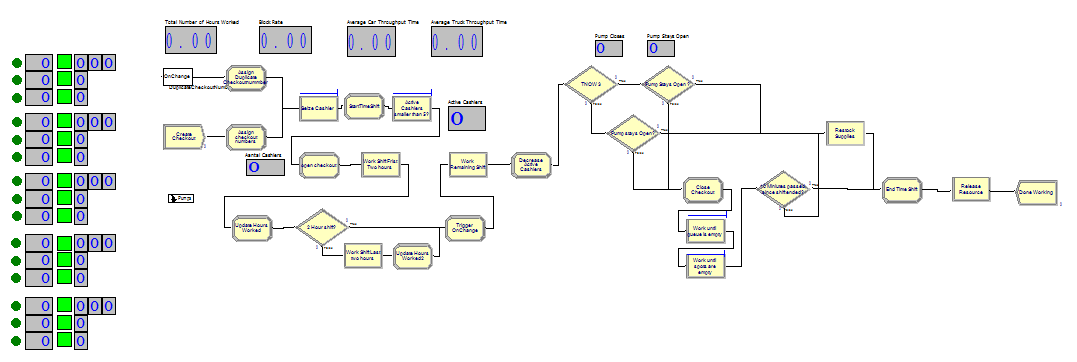
\includegraphics[scale=0.6]{images/model-description/main}
	\caption{Arena simulation model of the cashier management.}
	\label{fig:model-cashier}
\end{center}
\end{figure}

\begin{figure}[h!]
\begin{center}
	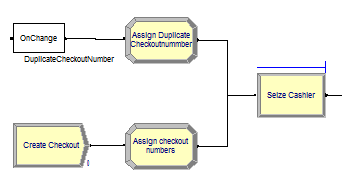
\includegraphics[scale=1]{images/model-description/checkout-creation.PNG}
	\caption{Modeling of the creation of checkouts.}
	\label{fig:createcheckouts}
\end{center}
\end{figure}

The second part of the model is shown in figure \ref{fig:seizeandopen}. 
When a cashier was seized the checkout moved to $StartTimeShift$ where the time the cashier started his shift is stored. 
After that the checkout moves on to $Active \ Cashiers \ smaller \ than \ 5?$. 
In this module it is checked whether the shift of the original checkout is finished before the duplicate checkout may move on. 
If this is not checked it is theoretically possible that both the original checkout and the duplicate checkout are manned. 
After this module all the associated lanes of the checkout are opened in $Open \ checkout$ and the first two hours of the shift in \textit{Work Shift First Two hours}. 
In this state the checkout will reside one hour and 59 minutes. 
The reason why a cashier works one minute less than two hours in this state is explained later. 

\begin{figure}[h!]
\begin{center}
	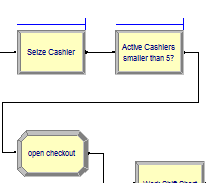
\includegraphics[scale=1]{images/model-description/seize-and-open.PNG}
	\caption{Modeling of the cashier seizing and checkout opening.}
	\label{fig:seizeandopen}
\end{center}
\end{figure}

The next part of the model is shown in figure \ref{fig:workshift}. 
After that the checkout has opened its associated lanes we first update the total amount of hours worked by cashiers. 
This is done in module \textit{Update Hours Worked}. 
We keep track of a variable called $TotalHoursWorked$ which represents the number of total hours worked by cashiers. 
This variable is updated in this module. 
This is also the reason why instead of working two hours in the former state the cashiers worked one minute less. 
In this way we know that just before the whole hour passes the variable is updated. 
This is important for the simulation since this simulation stops at a whole hour, so when this simulation stops the variable has just been updated.
After this module we check whether it's a 2 hour or a 4 hour shift. 
This is necessary because at the start of the simulation (0:00) cashiers from shift 12 are already working and they have only 2 hours left. 
So these cashiers will directly go to module \textit{Trigger OnChange}, where thee $OnChange$ module from figure \ref{fig:createcheckouts} creates a duplicate checkout.
The cashiers who work a normal shift will go to module \textit{Work Shift Last two hours} where a delay of two hours will represent working a shift for the same amount of time. 
We don't have to decrease the two hours with a minute this time, because after two hours we haven't reached a whole hour yet.
After this the total amount of hours worked will be updated again in \textit{Update Hours Worked2}. 
Next the cashiers work their remaining single minute in $Work \ Remaining \ Shift$. 
When the cashier is completely done with his regular shift we decrease the number of active cashiers so that possibly stuck duplicate checkout can continue from the $Active \ Cashiers \ smaller \ than \ 5?$ module we saw before.

\begin{figure}[h!]
\begin{center}
	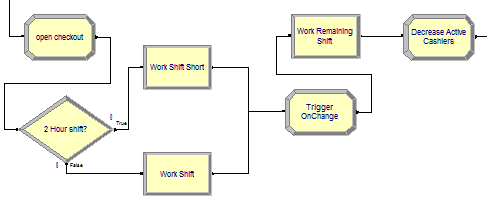
\includegraphics[scale=1]{images/model-description/work-shift.PNG}
	\caption{Modeling of the delay for the cashier working his/her shift.}
	\label{fig:workshift}
\end{center}
\end{figure}

\begin{figure}[]
\begin{center}
	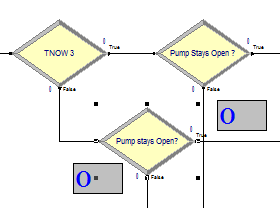
\includegraphics[scale=1]{images/model-description/determine-takeover.PNG}
	\caption{Modeling of the check whether a checkout is taken over.}
	\label{fig:determinetakeover}
\end{center}
\end{figure}

After the regular shift, we have to determine what will happen to the lanes and the cashier. 
Does he close the lanes and continue working at the checkout till the lanes are empty? 
Or does another cashier take over and can he go over to restocking the supplies? 
This is checked in the blocks displayed in figure \ref{fig:determinetakeover}. 
As you can see, the check whether someone takes over is split into two checks. 
This is due to a technicality issue: we have a global 1D array with 5 rows. 
Every row contains a time stamp. 
This time stamp represents the latest shift which started for that checkout. 
So in the upper right module $Pump \ Stays \ Open$ we check if the time stamp in the associated row in the array is newer than the expression "TNOW - 3.5", which means is the time stamp less than 3,5 hours old. 
If not the time stamp is the same as when the shift of the current cashier started and therefore we know the cashier has to close the lanes. 
If the time stamp is newer it means that another cashier is waiting to take over the shift. 
The technical problem we have is that for the first 3,5 hours we cannot use this expression, because it will always evaluate to true since there are no negative time stamps. 
Since shifts only start at whole hours we check if there has past more than 3 hours since the start of the simulation. 
In the bottom left $Pump \ stays \ Open$ module we just check if the new time stamp is larger or equal to 2, since that is the only shift of cashiers which can take over a checkout before we reach TNOW = 3. 

The last part of the cashier management is rather straightforward (figure \ref{fig:closerestockandrelease}): based on the previous decision, the checkout is closed after which the cashier works until the lane and checkout queue are both empty after which he restocks the supplies if less than 10 minutes have passed since the checkout was closed (which is calculated by setting a variable to the current time upon closing and comparing it to current time after the queue is emptied). 
Or the checkout does not close and the cashier immediately restocks the supplies.
After this the end time of the shift is determined and the total hours worked is again updated and the cashier is released and the checkout entity will be disposed.

\begin{figure}[h!]
\begin{center}
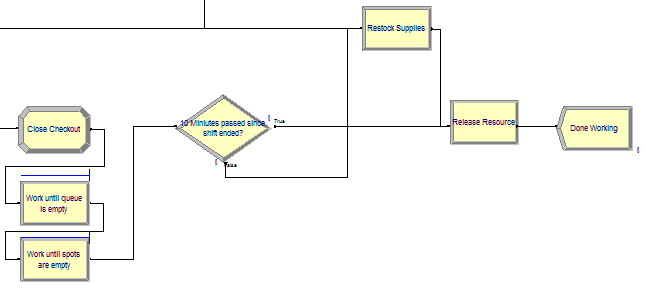
\includegraphics[scale=1]{images/model-description/close-restock-release.PNG}
	\caption{Modeling of the check whether a checkout is taken over.}
	\label{fig:closerestockandrelease}
\end{center}
\end{figure}

\clearpage
\subsection{Vehicle Management}\label{app:pumpdescription}
\begin{figure}[!ht]
\begin{center}
	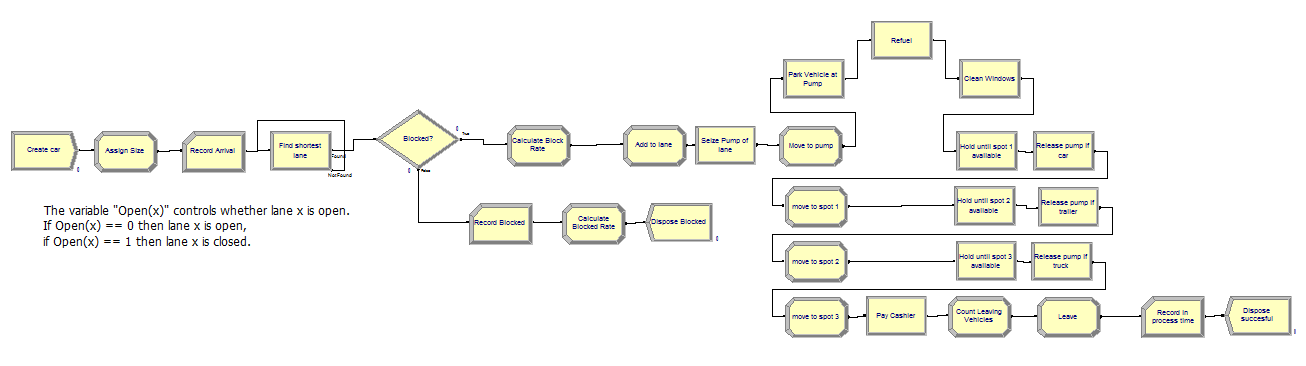
\includegraphics[scale=0.5]{images/model-description/pumps}
	\caption{Arena simulation model of the pump management.}
	\label{fig:modelpumps}
\end{center}
\end{figure}

This subsection describes the submodel where the vehicles are the entities that go through the system. 
First the model is described in general, after which each part will be described in detail. 
The whole submodel can be viewed in \autoref{fig:modelpumps}.

When a vehicle arrives, it is determined what type of vehicle it is. Then the vehicle queues up in the shortest lane if there is an open lane that has enough space for the vehicle (otherwise the vehicle is blocked). Then the vehicle parks, refuels, gets its windows cleaned and moves on to the payment queue. In this queue it moves forward whenever possible until it reaches the cashier, to which it pays and then leaves, recording the time it has been in the system.

We now discuss the model step-by-step in detail.
First the vehicle arrives, gets a size assigned, and its arrival is recorded in the system, see \autoref{fig:vehiclearrives}. 
Here we see the vehicle being created in \textit{Create car}, which keeps creating cars according to the Arrival Schedule, one at a time. 
Then in \textit{Assign Size} the arrival time and size attributes are set. Finally in \textit{Record Arrival} the arrivals are counted.

\begin{figure}[h]
\begin{center}
	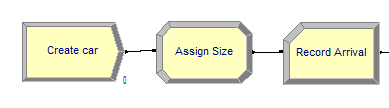
\includegraphics[scale=1]{images/model-description/vehicle-arrives.PNG}
	\caption{Modeling of the vehicle arriving.}
	\label{fig:vehiclearrives}
\end{center}
\end{figure}

Next, we describe choosing a lane, see the submodel in \autoref{fig:picklane}. In the leftmost block, \textit{Find shortest lane}, the minimum open lane is selected for this vehicle.
 After this, the block \textit{Check available space} determines whether or not the vehicle will be blocked. 
 It will be if the space in lane is insufficient for the current vehicle, or if the lane is closed. If the vehicle is blocked, this is recorded in \textit{Record Blocked} after which we dispose of it. 
 If the vehicle is not blocked, we add it to the lane by updating the space in the lane in \textit{Add to lane} and seizing the pump of the lane in \textit{Seize Pump of lane}.

\begin{figure}[h]
\begin{center}
	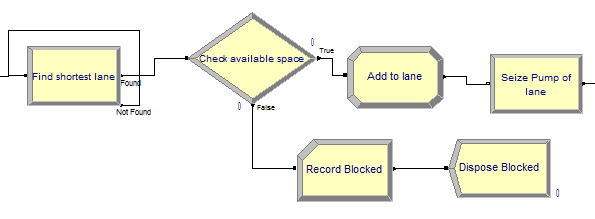
\includegraphics[scale=1]{images/model-description/pick-lane.PNG}
	\caption{Modeling of the vehicle picking a lane, checking if there is enough space, blocking if not and moving into the lane if yes.}
	\label{fig:picklane}
\end{center}
\end{figure}

In \autoref{fig:refuelprocess} we see how the vehicle moves to the pump (which shortens the queue by one), after which the tank process begins. 
This essentially consists of three delays: parking the vehicle in the \textit{Park Vehicle at Pump} block, refueling the vehicle (\textit{Refuel}) and cleaning the windows of the vehicle (\textit{Clean Windows}).

\begin{figure}[h]
\begin{center}
	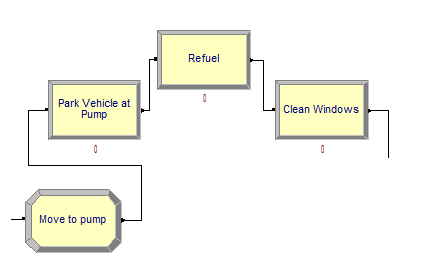
\includegraphics[scale=0.8]{images/model-description/refuel-process.PNG}
	\caption{Modeling of the vehicle moving to the pump, parking, refueling and cleaning its windows.}
	\label{fig:refuelprocess}
\end{center}
\end{figure}

Next, we discuss the queue in front of the cashier, see the submodel in \autoref{fig:cashierqueue} for this. 
There are three Hold blocks, which just hold the vehicle until the next spot frees up. 
Furthermore we have three release blocks, which release the pump when the vehicle moves away from it. 
For a car, this is when it moves into the first queue spot (as a car has length 1), for a car with trailer, when it moves to the second queue spot (as it has length 2) and for a truck when it moves to the third queue spot (length 3). 
Lastly we have three assign blocks which free up the lane behind the vehicle, depending on its length, and fill/free up the queue in front of the cashier likewise.

\begin{figure}[h!]
\begin{center}
	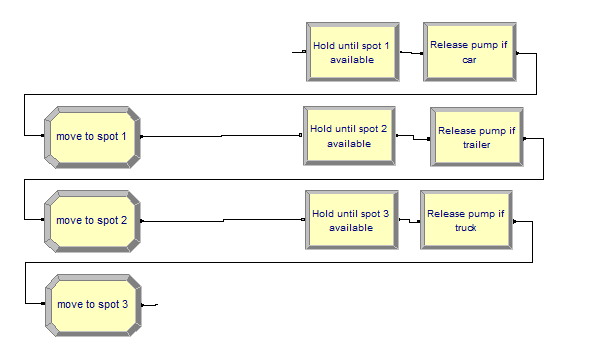
\includegraphics[scale=0.8]{images/model-description/cashier-queue.PNG}
	\caption{Modeling of the vehicle moving through the queue in front of the cashier.}
	\label{fig:cashierqueue}
\end{center}
\end{figure}

Finally we discuss the submodel shown in \autoref{fig:payleave}.
 The vehicle arrives at the cashier and pays (hold block). 
 Then it leaves, freeing up its remaining queue spots in front of the cashier (assign block \textit{Leave}).
 Then we record the time the vehicle has been in the process after which we dispose of it.

\begin{figure}[h!]
\begin{center}
	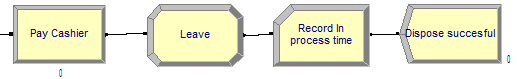
\includegraphics[scale=0.8]{images/model-description/pay-and-leave.PNG}
	\caption{Modeling of the vehicle paying and leaving the system.}
	\label{fig:payleave}
\end{center}
\end{figure}

\subsection{Resource schedules, variables and attributes}\label{app:resources}
There are 12 schedules to model the shifts, one for each of them.
To automate the process of finding a solution, these shifts do not contain fixed values but each contain a 4 hour period where 1 cashier is scheduled.
This number is then multiplied by one of the associated varibles A\_S1 $\ldots$ A\_S12.

Other important variables are \textit{Lane} and \textit{spots}.
The variable \textit{Lane} keeps track of each of the 15 lanes.
Variable \textit{spots} contains one field for every waiting spot for a cashier. 
